% ============================================================
%  CHƯƠNG II: THIẾT KẾ HỆ THỐNG
% ============================================================
\chapter{THIẾT KẾ HỆ THỐNG}
\label{chap:thiet_ke}

% ────────────────────────────────────────────────────────────
\section{Phân tích yêu cầu hệ thống}
\label{sec:phan_tich_yeu_cau}

% ── 1.1 Yêu cầu chức năng ───────────────────────────────────
\subsection{Yêu cầu chức năng (Functional Requirements)}
\label{subsec:yeu_cau_chuc_nang}

\subsubsection{Sơ đồ Use Case Tổng thể (Overview Use Case Diagram)}
Sơ đồ dưới đây minh họa các nhóm nghiệp vụ chính của ứng dụng CineFlow, được phân bổ
cho hai nhóm Tác nhân (Actors) cốt lõi: Người xem (User) và Quản trị viên (Admin). Hệ
thống Email Server tham gia gián tiếp trong luồng khôi phục mật khẩu.

\begin{figure}[H]
  \centering
  
\includegraphics[width=\textwidth, height=10cm, keepaspectratio]{outputs/usecase_diagram.png}
  \caption{Sơ đồ Use Case Tổng quát của ứng dụng CineFlow}
  \label{fig:usecase_diagram}
\end{figure}

\subsubsection{Đặc tả Use Case Chi tiết}
Dưới đây là đặc tả chi tiết 15 luồng nghiệp vụ cốt lõi (Use Cases) của hệ thống
CineFlow, được ánh xạ trực tiếp từ các endpoint của REST API và chia thành 5 nhóm
chức năng (Features) độc lập.


% ============================================================
%  NHÓM 1: Xác thực và Tài khoản (UC-01 .. UC-05)
% ============================================================
\subsubsection*{Nhóm 1: Xác thực và Tài khoản}

\begin{table}[H]
\renewcommand{\arraystretch}{1.3}
\centering
\begin{tabularx}{\textwidth}{|p{4.5cm}|X|}
\hline
\cellcolor{gray!15}\bfseries Mã Usecase & \textbf{UC-01} \\ \hline
\cellcolor{gray!15}\bfseries Tên Usecase & \textbf{Đăng ký tài khoản} \\ \hline
\cellcolor{gray!15}\bfseries Tác nhân (Actors) & Người xem (User) \\ \hline
\cellcolor{gray!15}\bfseries Mô tả ngắn & Người dùng tạo tài khoản mới trên CineFlow bằng email và mật khẩu. \\ \hline
\cellcolor{gray!15}\bfseries Điều kiện tiên quyết & Người dùng chưa đăng nhập, có kết nối Internet. \\ \hline
\cellcolor{gray!15}\bfseries Điều kiện đảm bảo & Tài khoản được tạo với vai trò \texttt{ROLE\_USER}, mật khẩu được băm trước khi lưu. \\ \hline
\cellcolor{gray!15}\bfseries Luồng sự kiện chính & 1. Người dùng nhập \texttt{username}, \texttt{email}, \texttt{password}.\newline 2. Hệ thống kiểm tra trùng lặp email/username.\newline 3. Hệ thống băm mật khẩu bằng BCrypt và lưu vào CSDL. \\ \hline
\cellcolor{gray!15}\bfseries Luồng rẽ nhánh & \textbf{Email đã tồn tại}: Hệ thống trả lỗi \textit{Email already exists}. \\ \hline
\cellcolor{gray!15}\bfseries Yêu cầu chức năng (FR) & $\diamond$ \textbf{FR\_01.1}: Mật khẩu phải có tối thiểu 6 ký tự.\newline $\diamond$ \textbf{FR\_01.2}: Mật khẩu không được lưu dưới dạng plaintext. \\ \hline
\end{tabularx}
\end{table}

\begin{table}[H]
\renewcommand{\arraystretch}{1.3}
\centering
\begin{tabularx}{\textwidth}{|p{4.5cm}|X|}
\hline
\cellcolor{gray!15}\bfseries Mã Usecase & \textbf{UC-02} \\ \hline
\cellcolor{gray!15}\bfseries Tên Usecase & \textbf{Đăng nhập hệ thống} \\ \hline
\cellcolor{gray!15}\bfseries Tác nhân (Actors) & Người xem (User), Quản trị viên (Admin) \\ \hline
\cellcolor{gray!15}\bfseries Mô tả ngắn & Người dùng đăng nhập bằng username và mật khẩu để nhận JWT. \\ \hline
\cellcolor{gray!15}\bfseries Điều kiện tiên quyết & Tài khoản đã được đăng ký. \\ \hline
\cellcolor{gray!15}\bfseries Điều kiện đảm bảo & Nhận về JWT có hạn 2 giờ; thông tin phiên được lưu vào \texttt{SharedPreferences}. \\ \hline
\cellcolor{gray!15}\bfseries Luồng sự kiện chính & 1. Người dùng nhập username/mật khẩu.\newline 2. Hệ thống đối chiếu mật khẩu băm trong CSDL.\newline 3. Hệ thống sinh JWT chứa \texttt{userId} và \texttt{role}, trả về cho client. \\ \hline
\cellcolor{gray!15}\bfseries Luồng rẽ nhánh & \textbf{Sai thông tin}: Báo lỗi \textit{Invalid username or password}. \\ \hline
\cellcolor{gray!15}\bfseries Yêu cầu chức năng (FR) & $\diamond$ \textbf{FR\_02.1}: JWT phải được ký bằng \texttt{JWT\_SECRET} từ biến môi trường.\newline $\diamond$ \textbf{FR\_02.2}: Token có thời hạn 2 giờ. \\ \hline
\end{tabularx}
\end{table}

\begin{table}[H]
\renewcommand{\arraystretch}{1.3}
\centering
\begin{tabularx}{\textwidth}{|p{4.5cm}|X|}
\hline
\cellcolor{gray!15}\bfseries Mã Usecase & \textbf{UC-03} \\ \hline
\cellcolor{gray!15}\bfseries Tên Usecase & \textbf{Quên mật khẩu} \\ \hline
\cellcolor{gray!15}\bfseries Tác nhân (Actors) & Người xem (User), Email Server \\ \hline
\cellcolor{gray!15}\bfseries Mô tả ngắn & Người dùng yêu cầu khôi phục mật khẩu qua email. \\ \hline
\cellcolor{gray!15}\bfseries Điều kiện tiên quyết & Không yêu cầu đăng nhập. \\ \hline
\cellcolor{gray!15}\bfseries Điều kiện đảm bảo & Hệ thống sinh \texttt{resetToken} có thời hạn và gửi link khôi phục vào email. \\ \hline
\cellcolor{gray!15}\bfseries Luồng sự kiện chính & 1. Người dùng nhập email.\newline 2. Hệ thống tạo \texttt{resetToken} ngẫu nhiên.\newline 3. Hệ thống gửi email chứa link kèm token qua SMTP. \\ \hline
\cellcolor{gray!15}\bfseries Luồng rẽ nhánh & \textbf{Email không tồn tại}: Trả về 200 OK nhưng không gửi mail để tránh lộ thông tin tài khoản. \\ \hline
\cellcolor{gray!15}\bfseries Yêu cầu chức năng (FR) & $\diamond$ \textbf{FR\_03.1}: \texttt{resetToken} chỉ có hiệu lực một lần duy nhất trong 30 phút. \\ \hline
\end{tabularx}
\end{table}

\begin{table}[H]
\renewcommand{\arraystretch}{1.3}
\centering
\begin{tabularx}{\textwidth}{|p{4.5cm}|X|}
\hline
\cellcolor{gray!15}\bfseries Mã Usecase & \textbf{UC-04} \\ \hline
\cellcolor{gray!15}\bfseries Tên Usecase & \textbf{Đặt lại mật khẩu} \\ \hline
\cellcolor{gray!15}\bfseries Tác nhân (Actors) & Người xem (User) \\ \hline
\cellcolor{gray!15}\bfseries Mô tả ngắn & Người dùng đặt mật khẩu mới sau khi xác thực qua \texttt{resetToken}. \\ \hline
\cellcolor{gray!15}\bfseries Điều kiện tiên quyết & Sở hữu \texttt{resetToken} hợp lệ, chưa hết hạn. \\ \hline
\cellcolor{gray!15}\bfseries Điều kiện đảm bảo & Mật khẩu mới được băm và lưu; token bị vô hiệu hoá. \\ \hline
\cellcolor{gray!15}\bfseries Luồng sự kiện chính & 1. Client kiểm tra token còn hiệu lực qua \texttt{GET /auth/validate-reset-token}.\newline 2. Người dùng nhập mật khẩu mới.\newline 3. Hệ thống băm mật khẩu, cập nhật CSDL, vô hiệu hoá token. \\ \hline
\cellcolor{gray!15}\bfseries Luồng rẽ nhánh & \textbf{Token hết hạn hoặc đã dùng}: Báo lỗi \textit{Reset token expired or already used}. \\ \hline
\cellcolor{gray!15}\bfseries Yêu cầu chức năng (FR) & $\diamond$ \textbf{FR\_04.1}: Sau khi đặt lại, mọi phiên đăng nhập cũ vẫn hợp lệ cho đến khi JWT hết hạn tự nhiên. \\ \hline
\end{tabularx}
\end{table}

\begin{table}[H]
\renewcommand{\arraystretch}{1.3}
\centering
\begin{tabularx}{\textwidth}{|p{4.5cm}|X|}
\hline
\cellcolor{gray!15}\bfseries Mã Usecase & \textbf{UC-05} \\ \hline
\cellcolor{gray!15}\bfseries Tên Usecase & \textbf{Đăng xuất} \\ \hline
\cellcolor{gray!15}\bfseries Tác nhân (Actors) & Người xem (User), Quản trị viên (Admin) \\ \hline
\cellcolor{gray!15}\bfseries Mô tả ngắn & Người dùng đăng xuất khỏi ứng dụng. \\ \hline
\cellcolor{gray!15}\bfseries Điều kiện tiên quyết & Người dùng đã đăng nhập. \\ \hline
\cellcolor{gray!15}\bfseries Điều kiện đảm bảo & Thông tin phiên trong \texttt{SharedPreferences} bị xoá; UI quay về trạng thái khách. \\ \hline
\cellcolor{gray!15}\bfseries Luồng sự kiện chính & 1. Người dùng bấm \textit{Đăng xuất} trong tab More.\newline 2. \texttt{AuthManager} xoá token, userId, username, role.\newline 3. UI \texttt{MoreFragment} tự cập nhật về trạng thái chưa đăng nhập. \\ \hline
\cellcolor{gray!15}\bfseries Luồng rẽ nhánh & Không có. \\ \hline
\cellcolor{gray!15}\bfseries Yêu cầu chức năng (FR) & $\diamond$ \textbf{FR\_05.1}: Đăng xuất chỉ là thao tác phía client; backend là stateless. \\ \hline
\end{tabularx}
\end{table}


% ============================================================
%  NHÓM 2: Khám phá Nội dung (UC-06 .. UC-10)
% ============================================================
\subsubsection*{Nhóm 2: Khám phá Nội dung}

\begin{table}[H]
\renewcommand{\arraystretch}{1.3}
\centering
\begin{tabularx}{\textwidth}{|p{4.5cm}|X|}
\hline
\cellcolor{gray!15}\bfseries Mã Usecase & \textbf{UC-06} \\ \hline
\cellcolor{gray!15}\bfseries Tên Usecase & \textbf{Xem trang chủ} \\ \hline
\cellcolor{gray!15}\bfseries Tác nhân (Actors) & Người xem (User), Khách (Guest) \\ \hline
\cellcolor{gray!15}\bfseries Mô tả ngắn & Người dùng xem trang chủ với nhiều khu vực nội dung (banner, phim mới, sự kiện thể thao, series, phim trong ngày). \\ \hline
\cellcolor{gray!15}\bfseries Điều kiện tiên quyết & Không yêu cầu đăng nhập. \\ \hline
\cellcolor{gray!15}\bfseries Điều kiện đảm bảo & Trang chủ hiển thị đầy đủ năm khu vực nội dung. \\ \hline
\cellcolor{gray!15}\bfseries Luồng sự kiện chính & 1. \texttt{HomeFragment} gọi \texttt{GET /films/home}.\newline 2. Backend trả về object chứa \texttt{banners}, \texttt{newReleases}, \texttt{sportEvents}, \texttt{hotSeries}, \texttt{dailyMovies}.\newline 3. Client render từng khu vực vào \texttt{RecyclerView} tương ứng. \\ \hline
\cellcolor{gray!15}\bfseries Luồng rẽ nhánh & \textbf{Mất kết nối}: Hiển thị thông báo lỗi và nút \textit{Thử lại}. \\ \hline
\cellcolor{gray!15}\bfseries Yêu cầu chức năng (FR) & $\diamond$ \textbf{FR\_06.1}: Trang chủ phải hiển thị trong $\leq$ 2 giây với cache ảnh Glide. \\ \hline
\end{tabularx}
\end{table}

\begin{table}[H]
\renewcommand{\arraystretch}{1.3}
\centering
\begin{tabularx}{\textwidth}{|p{4.5cm}|X|}
\hline
\cellcolor{gray!15}\bfseries Mã Usecase & \textbf{UC-07} \\ \hline
\cellcolor{gray!15}\bfseries Tên Usecase & \textbf{Xem chi tiết phim} \\ \hline
\cellcolor{gray!15}\bfseries Tác nhân (Actors) & Người xem (User) \\ \hline
\cellcolor{gray!15}\bfseries Mô tả ngắn & Người dùng xem mô tả chi tiết, trailer và danh sách tập của một phim. \\ \hline
\cellcolor{gray!15}\bfseries Điều kiện tiên quyết & Người dùng đã chọn một phim từ trang chủ hoặc kết quả tìm kiếm. \\ \hline
\cellcolor{gray!15}\bfseries Điều kiện đảm bảo & \texttt{FilmDetailActivity} hiển thị đầy đủ thông tin phim và danh sách \texttt{Episode}. \\ \hline
\cellcolor{gray!15}\bfseries Luồng sự kiện chính & 1. Client gọi \texttt{GET /films/\{id\}}.\newline 2. Backend trả về \texttt{Film} kèm danh sách \texttt{Episode}.\newline 3. UI render mô tả, ảnh thumbnail và danh sách tập. \\ \hline
\cellcolor{gray!15}\bfseries Luồng rẽ nhánh & \textbf{Không tìm thấy phim}: Backend trả 404, client hiển thị thông báo \textit{Phim không tồn tại}. \\ \hline
\cellcolor{gray!15}\bfseries Yêu cầu chức năng (FR) & $\diamond$ \textbf{FR\_07.1}: Với phim lẻ (\texttt{SINGLE}), hệ thống tự sinh một \texttt{Episode} mặc định để tái sử dụng luồng phát. \\ \hline
\end{tabularx}
\end{table}

\begin{table}[H]
\renewcommand{\arraystretch}{1.3}
\centering
\begin{tabularx}{\textwidth}{|p{4.5cm}|X|}
\hline
\cellcolor{gray!15}\bfseries Mã Usecase & \textbf{UC-08} \\ \hline
\cellcolor{gray!15}\bfseries Tên Usecase & \textbf{Phát video} \\ \hline
\cellcolor{gray!15}\bfseries Tác nhân (Actors) & Người xem (User) \\ \hline
\cellcolor{gray!15}\bfseries Mô tả ngắn & Người dùng phát phim lẻ, một tập của series, hoặc sự kiện trực tiếp. \\ \hline
\cellcolor{gray!15}\bfseries Điều kiện tiên quyết & Đã chọn một \texttt{Episode}/phim cụ thể, có kết nối Internet. \\ \hline
\cellcolor{gray!15}\bfseries Điều kiện đảm bảo & Video bắt đầu phát trong \texttt{PlayerActivity}. \\ \hline
\cellcolor{gray!15}\bfseries Luồng sự kiện chính & 1. Client mở \texttt{PlayerActivity} với \texttt{videoUrl}.\newline 2. ExoPlayer khởi tạo \texttt{MediaItem} và bắt đầu prepare.\newline 3. Player phát video, hiển thị thanh điều khiển. \\ \hline
\cellcolor{gray!15}\bfseries Luồng rẽ nhánh & \textbf{URL không khả dụng}: Player phát ra \texttt{Player.Listener.onPlayerError}, UI hiển thị lỗi và nút \textit{Thử lại}. \\ \hline
\cellcolor{gray!15}\bfseries Yêu cầu chức năng (FR) & $\diamond$ \textbf{FR\_08.1}: Player phải giải phóng tài nguyên trong \texttt{onDestroy()} để tránh rò rỉ bộ nhớ. \\ \hline
\end{tabularx}
\end{table}

\begin{table}[H]
\renewcommand{\arraystretch}{1.3}
\centering
\begin{tabularx}{\textwidth}{|p{4.5cm}|X|}
\hline
\cellcolor{gray!15}\bfseries Mã Usecase & \textbf{UC-09} \\ \hline
\cellcolor{gray!15}\bfseries Tên Usecase & \textbf{Xem video ngắn (Shorts)} \\ \hline
\cellcolor{gray!15}\bfseries Tác nhân (Actors) & Người xem (User) \\ \hline
\cellcolor{gray!15}\bfseries Mô tả ngắn & Người dùng cuộn dọc xem các video ngắn, tự động phát/dừng theo vị trí cuộn. \\ \hline
\cellcolor{gray!15}\bfseries Điều kiện tiên quyết & Có kết nối Internet. \\ \hline
\cellcolor{gray!15}\bfseries Điều kiện đảm bảo & Mỗi lần cuộn chỉ có duy nhất một video đang phát; các video còn lại dừng. \\ \hline
\cellcolor{gray!15}\bfseries Luồng sự kiện chính & 1. \texttt{ShortsFragment} gọi \texttt{GET /films/shorts}.\newline 2. Client gắn danh sách vào \texttt{ViewPager2} dọc.\newline 3. Khi page change, video đang hiển thị tự play, video trước/sau pause. \\ \hline
\cellcolor{gray!15}\bfseries Luồng rẽ nhánh & \textbf{Hết danh sách}: Hiển thị placeholder \textit{Đã hết shorts}. \\ \hline
\cellcolor{gray!15}\bfseries Yêu cầu chức năng (FR) & $\diamond$ \textbf{FR\_09.1}: Bộ nhớ ExoPlayer phải được tái sử dụng để tránh tạo mới mỗi lần cuộn. \\ \hline
\end{tabularx}
\end{table}

\begin{table}[H]
\renewcommand{\arraystretch}{1.3}
\centering
\begin{tabularx}{\textwidth}{|p{4.5cm}|X|}
\hline
\cellcolor{gray!15}\bfseries Mã Usecase & \textbf{UC-10} \\ \hline
\cellcolor{gray!15}\bfseries Tên Usecase & \textbf{Xem lịch Premier League} \\ \hline
\cellcolor{gray!15}\bfseries Tác nhân (Actors) & Người xem (User) \\ \hline
\cellcolor{gray!15}\bfseries Mô tả ngắn & Người dùng xem lịch thi đấu Ngoại hạng Anh, có thể lọc theo mùa giải và theo ngày. \\ \hline
\cellcolor{gray!15}\bfseries Điều kiện tiên quyết & Có kết nối Internet. \\ \hline
\cellcolor{gray!15}\bfseries Điều kiện đảm bảo & Lịch hiển thị theo giờ Việt Nam, đã quy đổi từ UTC. \\ \hline
\cellcolor{gray!15}\bfseries Luồng sự kiện chính & 1. \texttt{PremierLeagueFragment} chọn mùa giải.\newline 2. \texttt{PremierLeagueRepository} gọi backend với tham số \texttt{season}, \texttt{date}.\newline 3. Backend trả về danh sách trận; client render theo nhóm ngày. \\ \hline
\cellcolor{gray!15}\bfseries Luồng rẽ nhánh & \textbf{Không có trận nào}: Hiển thị thông báo \textit{Chưa có trận đấu trong ngày}. \\ \hline
\cellcolor{gray!15}\bfseries Yêu cầu chức năng (FR) & $\diamond$ \textbf{FR\_10.1}: Mọi mốc thời gian phải được hiển thị theo múi giờ \texttt{Asia/Ho\_Chi\_Minh}. \\ \hline
\end{tabularx}
\end{table}


% ============================================================
%  NHÓM 3: Quản trị Phim (UC-11 .. UC-14)
% ============================================================
\subsubsection*{Nhóm 3: Quản trị Phim}

\begin{table}[H]
\renewcommand{\arraystretch}{1.3}
\centering
\begin{tabularx}{\textwidth}{|p{4.5cm}|X|}
\hline
\cellcolor{gray!15}\bfseries Mã Usecase & \textbf{UC-11} \\ \hline
\cellcolor{gray!15}\bfseries Tên Usecase & \textbf{Xem Dashboard quản trị} \\ \hline
\cellcolor{gray!15}\bfseries Tác nhân (Actors) & Quản trị viên (Admin) \\ \hline
\cellcolor{gray!15}\bfseries Mô tả ngắn & Admin truy cập bảng điều khiển với các chỉ số tổng quan và liên kết tới các khu vực quản lý. \\ \hline
\cellcolor{gray!15}\bfseries Điều kiện tiên quyết & Tài khoản có vai trò \texttt{ROLE\_ADMIN}. \\ \hline
\cellcolor{gray!15}\bfseries Điều kiện đảm bảo & \texttt{AdminDashboardActivity} hiển thị các thẻ Films/Users/Categories/Stats. \\ \hline
\cellcolor{gray!15}\bfseries Luồng sự kiện chính & 1. \texttt{MoreFragment} kiểm tra \texttt{AuthManager.isAdmin()}.\newline 2. Hiển thị card \textit{Admin Panel}.\newline 3. Mở \texttt{AdminDashboardActivity} qua \texttt{Intent}. \\ \hline
\cellcolor{gray!15}\bfseries Luồng rẽ nhánh & \textbf{User thường}: Card Admin Panel bị ẩn, không thể truy cập. \\ \hline
\cellcolor{gray!15}\bfseries Yêu cầu chức năng (FR) & $\diamond$ \textbf{FR\_11.1}: Việc phân quyền ở client chỉ là tầng UI; backend phải kiểm tra lại role ở mọi endpoint admin. \\ \hline
\end{tabularx}
\end{table}

\begin{table}[H]
\renewcommand{\arraystretch}{1.3}
\centering
\begin{tabularx}{\textwidth}{|p{4.5cm}|X|}
\hline
\cellcolor{gray!15}\bfseries Mã Usecase & \textbf{UC-12} \\ \hline
\cellcolor{gray!15}\bfseries Tên Usecase & \textbf{Tạo phim mới} \\ \hline
\cellcolor{gray!15}\bfseries Tác nhân (Actors) & Quản trị viên (Admin) \\ \hline
\cellcolor{gray!15}\bfseries Mô tả ngắn & Admin tạo một phim mới với đầy đủ các thuộc tính: tiêu đề, mô tả, thumbnail, trailer, loại phim. \\ \hline
\cellcolor{gray!15}\bfseries Điều kiện tiên quyết & Đã đăng nhập với vai trò Admin. \\ \hline
\cellcolor{gray!15}\bfseries Điều kiện đảm bảo & Phim mới được lưu vào CSDL và xuất hiện trong \texttt{AdminFilmListActivity}. \\ \hline
\cellcolor{gray!15}\bfseries Luồng sự kiện chính & 1. Admin bấm FAB \textit{Tạo mới} trong \texttt{AdminFilmListActivity}.\newline 2. \texttt{FilmFormDialogFragment} mở, Admin điền form.\newline 3. Client gọi \texttt{POST /admin/films}.\newline 4. Danh sách phim tự refresh. \\ \hline
\cellcolor{gray!15}\bfseries Luồng rẽ nhánh & \textbf{Thiếu trường bắt buộc}: Backend trả \textit{Validation Failed (400)}; client hiển thị lỗi tại field tương ứng. \\ \hline
\cellcolor{gray!15}\bfseries Yêu cầu chức năng (FR) & $\diamond$ \textbf{FR\_12.1}: Trường \texttt{title} và \texttt{type} là bắt buộc. \\ \hline
\end{tabularx}
\end{table}

\begin{table}[H]
\renewcommand{\arraystretch}{1.3}
\centering
\begin{tabularx}{\textwidth}{|p{4.5cm}|X|}
\hline
\cellcolor{gray!15}\bfseries Mã Usecase & \textbf{UC-13} \\ \hline
\cellcolor{gray!15}\bfseries Tên Usecase & \textbf{Cập nhật phim} \\ \hline
\cellcolor{gray!15}\bfseries Tác nhân (Actors) & Quản trị viên (Admin) \\ \hline
\cellcolor{gray!15}\bfseries Mô tả ngắn & Admin sửa thông tin một phim đã có. \\ \hline
\cellcolor{gray!15}\bfseries Điều kiện tiên quyết & Phim cần sửa tồn tại trong CSDL. \\ \hline
\cellcolor{gray!15}\bfseries Điều kiện đảm bảo & Phim được cập nhật, ứng dụng người dùng nhìn thấy ngay ở lần gọi API tiếp theo. \\ \hline
\cellcolor{gray!15}\bfseries Luồng sự kiện chính & 1. Admin bấm item phim trong danh sách $\rightarrow$ chọn \textit{Sửa}.\newline 2. \texttt{FilmFormDialogFragment} mở với dữ liệu hiện tại.\newline 3. Admin sửa và bấm \textit{Lưu}.\newline 4. Client gọi \texttt{PUT /admin/films/\{id\}}. \\ \hline
\cellcolor{gray!15}\bfseries Luồng rẽ nhánh & \textbf{Phim không tồn tại}: Backend trả 404; client hiển thị thông báo và đóng dialog. \\ \hline
\cellcolor{gray!15}\bfseries Yêu cầu chức năng (FR) & $\diamond$ \textbf{FR\_13.1}: Các tập (\texttt{Episode}) của phim không bị xoá khi sửa thông tin phim. \\ \hline
\end{tabularx}
\end{table}

\begin{table}[H]
\renewcommand{\arraystretch}{1.3}
\centering
\begin{tabularx}{\textwidth}{|p{4.5cm}|X|}
\hline
\cellcolor{gray!15}\bfseries Mã Usecase & \textbf{UC-14} \\ \hline
\cellcolor{gray!15}\bfseries Tên Usecase & \textbf{Xoá phim} \\ \hline
\cellcolor{gray!15}\bfseries Tác nhân (Actors) & Quản trị viên (Admin) \\ \hline
\cellcolor{gray!15}\bfseries Mô tả ngắn & Admin xoá một phim khỏi hệ thống. \\ \hline
\cellcolor{gray!15}\bfseries Điều kiện tiên quyết & Phim cần xoá tồn tại. \\ \hline
\cellcolor{gray!15}\bfseries Điều kiện đảm bảo & Phim và các \texttt{Episode} liên quan bị xoá khỏi CSDL theo cơ chế cascade. \\ \hline
\cellcolor{gray!15}\bfseries Luồng sự kiện chính & 1. Admin bấm icon xoá trên một item phim.\newline 2. Dialog xác nhận hiển thị.\newline 3. Admin xác nhận; client gọi \texttt{DELETE /admin/films/\{id\}}.\newline 4. Danh sách tự refresh. \\ \hline
\cellcolor{gray!15}\bfseries Luồng rẽ nhánh & \textbf{Phim đang được tham chiếu}: Backend trả lỗi ràng buộc khoá ngoại; client hiển thị thông báo. \\ \hline
\cellcolor{gray!15}\bfseries Yêu cầu chức năng (FR) & $\diamond$ \textbf{FR\_14.1}: Thao tác xoá là không thể hoàn tác. \\ \hline
\end{tabularx}
\end{table}


% ============================================================
%  NHÓM 4: Quản lý Danh mục (UC-15)
% ============================================================
\subsubsection*{Nhóm 4: Quản lý Danh mục}

\begin{table}[H]
\renewcommand{\arraystretch}{1.3}
\centering
\begin{tabularx}{\textwidth}{|p{4.5cm}|X|}
\hline
\cellcolor{gray!15}\bfseries Mã Usecase & \textbf{UC-15} \\ \hline
\cellcolor{gray!15}\bfseries Tên Usecase & \textbf{Quản lý danh mục thể loại} \\ \hline
\cellcolor{gray!15}\bfseries Tác nhân (Actors) & Quản trị viên (Admin) \\ \hline
\cellcolor{gray!15}\bfseries Mô tả ngắn & Admin thêm, sửa, xoá các danh mục (Category) để phân loại phim. \\ \hline
\cellcolor{gray!15}\bfseries Điều kiện tiên quyết & Đã đăng nhập với vai trò Admin. \\ \hline
\cellcolor{gray!15}\bfseries Điều kiện đảm bảo & Danh sách \texttt{Category} được cập nhật và phản ánh trên trang chủ ở lần gọi tiếp theo. \\ \hline
\cellcolor{gray!15}\bfseries Luồng sự kiện chính & 1. Admin mở khu vực \textit{Categories} từ Dashboard.\newline 2. Thực hiện thao tác CRUD trên danh sách.\newline 3. Client gọi endpoint \texttt{/admin/categories} tương ứng. \\ \hline
\cellcolor{gray!15}\bfseries Luồng rẽ nhánh & \textbf{Xoá danh mục đang có phim}: Backend chặn xoá và trả lỗi; Admin phải gỡ liên kết phim trước. \\ \hline
\cellcolor{gray!15}\bfseries Yêu cầu chức năng (FR) & $\diamond$ \textbf{FR\_15.1}: Tên danh mục là duy nhất trong toàn hệ thống. \\ \hline
\end{tabularx}
\end{table}


% ============================================================
%  NHÓM 5: Tương tác và Cá nhân hóa (UC-16 .. UC-19)
% ============================================================
\subsubsection*{Nhóm 5: Tương tác và Cá nhân hóa}

\begin{table}[H]
\renewcommand{\arraystretch}{1.3}
\centering
\begin{tabularx}{\textwidth}{|p{4.5cm}|X|}
\hline
\cellcolor{gray!15}\bfseries Mã Usecase & \textbf{UC-16} \\ \hline
\cellcolor{gray!15}\bfseries Tên Usecase & \textbf{Đánh dấu phim yêu thích} \\ \hline
\cellcolor{gray!15}\bfseries Tác nhân (Actors) & Người xem (User) \\ \hline
\cellcolor{gray!15}\bfseries Mô tả ngắn & Người dùng thêm hoặc xóa một bộ phim khỏi danh sách yêu thích cá nhân. \\ \hline
\cellcolor{gray!15}\bfseries Điều kiện tiên quyết & Người dùng đã đăng nhập vào hệ thống. \\ \hline
\cellcolor{gray!15}\bfseries Điều kiện đảm bảo & Trạng thái yêu thích được lưu trữ đồng bộ dưới cơ sở dữ liệu và hiển thị đúng trên UI. \\ \hline
\cellcolor{gray!15}\bfseries Luồng sự kiện chính & 1. Người dùng bấm nút "Thêm vào yêu thích" trên màn hình chi tiết phim.\newline 2. Client gửi yêu cầu \texttt{POST /favorites/\{filmId\}} hoặc \texttt{DELETE /favorites/\{filmId\}}.\newline 3. Hệ thống cập nhật bảng \texttt{favorites} trong CSDL và phản hồi thành công.\newline 4. UI cập nhật màu sắc và văn bản của nút tương ứng. \\ \hline
\cellcolor{gray!15}\bfseries Luồng rẽ nhánh & \textbf{Chưa đăng nhập}: Hệ thống chuyển hướng người dùng tới màn hình đăng nhập. \\ \hline
\cellcolor{gray!15}\bfseries Yêu cầu chức năng (FR) & $\diamond$ \textbf{FR\_16.1}: Phải hiển thị đúng danh sách phim yêu thích cá nhân tại tab Favorites. \\ \hline
\end{tabularx}
\end{table}

\begin{table}[H]
\renewcommand{\arraystretch}{1.3}
\centering
\begin{tabularx}{\textwidth}{|p{4.5cm}|X|}
\hline
\cellcolor{gray!15}\bfseries Mã Usecase & \textbf{UC-17} \\ \hline
\cellcolor{gray!15}\bfseries Tên Usecase & \textbf{Bình luận phim và video ngắn} \\ \hline
\cellcolor{gray!15}\bfseries Tác nhân (Actors) & Người xem (User) \\ \hline
\cellcolor{gray!15}\bfseries Mô tả ngắn & Người dùng viết và gửi bình luận dưới các phim hoặc video ngắn, cũng như xem các bình luận khác. \\ \hline
\cellcolor{gray!15}\bfseries Điều kiện tiên quyết & Có kết nối Internet; Đã đăng nhập để gửi bình luận. \\ \hline
\cellcolor{gray!15}\bfseries Điều kiện đảm bảo & Bình luận mới được hiển thị ngay lập tức ở đầu danh sách bình luận. \\ \hline
\cellcolor{gray!15}\bfseries Luồng sự kiện chính & 1. Người dùng cuộn tới phần bình luận, hệ thống gọi \texttt{GET /films/\{filmId\}/comments}.\newline 2. Người dùng nhập văn bản và nhấn gửi.\newline 3. Client gọi \texttt{POST /films/\{filmId\}/comments}.\newline 4. Hệ thống lưu bình luận vào bảng \texttt{film\_comments} và thêm vào giao diện. \\ \hline
\cellcolor{gray!15}\bfseries Luồng rẽ nhánh & \textbf{Chưa đăng nhập}: Ẩn ô nhập nội dung bình luận, hiển thị liên kết đăng nhập. \\ \hline
\cellcolor{gray!15}\bfseries Yêu cầu chức năng (FR) & $\diamond$ \textbf{FR\_17.1}: Nội dung bình luận không được để trống.\newline $\diamond$ \textbf{FR\_17.2}: Người dùng chỉ có quyền xóa bình luận do chính mình tạo ra. \\ \hline
\end{tabularx}
\end{table}

\begin{table}[H]
\renewcommand{\arraystretch}{1.3}
\centering
\begin{tabularx}{\textwidth}{|p{4.5cm}|X|}
\hline
\cellcolor{gray!15}\bfseries Mã Usecase & \textbf{UC-18} \\ \hline
\cellcolor{gray!15}\bfseries Tên Usecase & \textbf{Lưu lịch sử và tiến trình xem} \\ \hline
\cellcolor{gray!15}\bfseries Tác nhân (Actors) & Người xem (User) \\ \hline
\cellcolor{gray!15}\bfseries Mô tả ngắn & Hệ thống tự động ghi nhận lại tiến trình phát video (vị trí giây cuối cùng) của người dùng để tiếp tục phát ở lần sau. \\ \hline
\cellcolor{gray!15}\bfseries Điều kiện tiên quyết & Người dùng đang phát một tập phim. \\ \hline
\cellcolor{gray!15}\bfseries Điều kiện đảm bảo & Tiến trình được cập nhật định kỳ lên backend và lưu trữ tại bảng \texttt{watch\_history}. \\ \hline
\cellcolor{gray!15}\bfseries Luồng sự kiện chính & 1. Khi người dùng phát video, ExoPlayer ghi nhận thời điểm dừng phát (hoặc gửi định kỳ).\newline 2. Client gọi \texttt{PUT /watch-history/\{episodeId\}} kèm vị trí giây.\newline 3. Hệ thống lưu/cập nhật thông tin vào bảng \texttt{watch\_history}.\newline 4. Ở lần tiếp theo người dùng mở lại phim này, hệ thống gợi ý tiếp tục phát từ điểm đã dừng. \\ \hline
\cellcolor{gray!15}\bfseries Luồng rẽ nhánh & Không có. \\ \hline
\cellcolor{gray!15}\bfseries Yêu cầu chức năng (FR) & $\diamond$ \textbf{FR\_18.1}: Vị trí tiến trình lưu phải đảm bảo không vượt quá tổng thời lượng của tập phim. \\ \hline
\end{tabularx}
\end{table}

\begin{table}[H]
\renewcommand{\arraystretch}{1.3}
\centering
\begin{tabularx}{\textwidth}{|p{4.5cm}|X|}
\hline
\cellcolor{gray!15}\bfseries Mã Usecase & \textbf{UC-19} \\ \hline
\cellcolor{gray!15}\bfseries Tên Usecase & \textbf{Quản lý hồ sơ người dùng} \\ \hline
\cellcolor{gray!15}\bfseries Tác nhân (Actors) & Người xem (User) \\ \hline
\cellcolor{gray!15}\bfseries Mô tả ngắn & Người dùng xem thông tin tài khoản cá nhân, đổi mật khẩu hoặc cập nhật họ tên. \\ \hline
\cellcolor{gray!15}\bfseries Điều kiện tiên quyết & Người dùng đã đăng nhập. \\ \hline
\cellcolor{gray!15}\bfseries Điều kiện đảm bảo & Thông tin cập nhật thành công được đồng bộ vào bảng \texttt{users} và cập nhật trực tiếp trên giao diện Client. \\ \hline
\cellcolor{gray!15}\bfseries Luồng sự kiện chính & 1. Người dùng mở tab More, chọn sửa hồ sơ.\newline 2. Hệ thống hiển thị thông tin lấy từ \texttt{GET /user/me}.\newline 3. Người dùng cập nhật họ tên hoặc đổi mật khẩu và nhấn Lưu.\newline 4. Client gọi \texttt{PUT /user/profile} hoặc \texttt{POST /user/change-password} để đồng bộ dữ liệu. \\ \hline
\cellcolor{gray!15}\bfseries Luồng rẽ nhánh & \textbf{Đổi mật khẩu sai mật khẩu cũ}: Backend trả lỗi xác thực mật khẩu; client hiển thị thông báo lỗi. \\ \hline
\cellcolor{gray!15}\bfseries Yêu cầu chức năng (FR) & $\diamond$ \textbf{FR\_19.1}: Mật khẩu mới thay đổi phải tuân thủ độ dài tối thiểu 6 ký tự. \\ \hline
\end{tabularx}
\end{table}



% ── 1.2 Yêu cầu phi chức năng ───────────────────────────────
\subsection{Yêu cầu phi chức năng (Non-Functional Requirements)}
\label{subsec:yeu_cau_phi_chuc_nang}

Bảng~\ref{tab:nfr} tổng hợp các yêu cầu phi chức năng của hệ thống CineFlow, chia
theo 6 thuộc tính chất lượng.

\begin{table}[H]
  \centering
  \caption{Yêu cầu phi chức năng của hệ thống CineFlow}
  \label{tab:nfr}
  \renewcommand{\arraystretch}{1.4}
  \begin{tabularx}{\textwidth}{|l|X|X|}
    \hline
    \textbf{Thuộc tính}      & \textbf{Yêu cầu} & \textbf{Giải pháp kỹ thuật} \\
    \hline
    \textbf{Hiệu năng}       &
    Thời gian phản hồi API $\leq$ 500ms (p95) cho các endpoint nghiệp vụ chính. Video
    bắt đầu phát trong $\leq$ 3 giây kể từ khi người dùng bấm Play. &
    Backend tách Repository -- Service -- Controller; Android client tải bất đồng bộ
    qua Retrofit + OkHttp; ExoPlayer với HLS adaptive bitrate. \\
    \hline
    \textbf{Khả năng mở rộng} &
    Ứng dụng có thể bổ sung loại nội dung mới (Series, Live, Shorts) mà không phải
    sửa đổi cấu trúc cốt lõi. &
    Mô hình dữ liệu thống nhất quanh \texttt{Film} với enum \texttt{FilmType}; backend
    phân lớp ba tầng giúp thêm endpoint mới mà không phá vỡ tầng dữ liệu. \\
    \hline
    \textbf{Tính nhất quán dữ liệu} &
    Schema cơ sở dữ liệu của tất cả thành viên trong nhóm phải luôn đồng bộ. Các thao
    tác CRUD trên Admin Panel phản ánh ngay xuống ứng dụng người dùng. &
    Flyway Migrations quản lý schema theo phiên bản. Backend đọc/ghi cùng một
    PostgreSQL nên không có khoảng trễ đồng bộ. \\
    \hline
    \textbf{Bảo mật} &
    Mọi endpoint quản trị phải xác thực. Mật khẩu không được lưu dưới dạng plaintext.
    Token đăng nhập phải có hạn sử dụng. &
    JWT Bearer Token với chữ ký HMAC-SHA256, thời hạn 2 giờ. Mật khẩu băm bằng BCrypt.
    Android client lưu token trong \texttt{SharedPreferences} ở chế độ private. \\
    \hline
    \textbf{Tính sẵn sàng} &
    Ứng dụng phải xử lý được trường hợp mất mạng tạm thời mà không bị treo (ANR --
    Application Not Responding). &
    Mọi lời gọi mạng dùng Retrofit \texttt{enqueue} bất đồng bộ trên luồng nền; UI
    cập nhật qua \texttt{LiveData} lifecycle-aware; hiển thị trạng thái lỗi thân thiện
    khi mất kết nối. \\
    \hline
    \textbf{Bảo trì \& vận hành} &
    Schema database chỉ được thay đổi qua migration, không sửa trực tiếp. Mã nguồn
    Android tuân thủ kiến trúc phân lớp, dễ kiểm thử. &
    Flyway cho phía backend; \texttt{BaseFragment} chuẩn hoá lifecycle Android; tất
    cả Fragment tuân theo luồng \texttt{getLayoutId} $\rightarrow$ \texttt{initViews}
    $\rightarrow$ \texttt{initData}. \\
    \hline
  \end{tabularx}
\end{table}


% ────────────────────────────────────────────────────────────
\section{Thiết kế lược đồ dữ liệu}
\label{sec:luoc_do_du_lieu}

Khác với các hệ thống Microservices theo mô hình Database-per-Service, CineFlow là
một ứng dụng đơn khối (Monolith) ở phía backend nên toàn bộ dữ liệu được lưu tập
trung trong một cơ sở dữ liệu PostgreSQL duy nhất. Lược đồ dữ liệu được tổ chức quanh
ba nhóm thực thể chính: \textit{Tài khoản \& Gói cước}, \textit{Nội dung phim} và
\textit{Tương tác người dùng}.

\subsection{Nhóm Tài khoản và Gói cước}

\begin{itemize}
  \item \textbf{User (Aggregate Root):} Lưu trữ thông tin tài khoản cốt lõi như
  \texttt{username}, \texttt{email}, \texttt{password} (đã băm BCrypt) và
  \texttt{role}. Trường \texttt{role} sử dụng kiểu enum \texttt{UserRole}
  (\textit{ROLE\_USER}, \textit{ROLE\_ADMIN}) để phân biệt hai nhóm người dùng ngay
  trong cùng một bảng -- thiết kế đơn giản nhưng đủ cho phạm vi đồ án.

  \item \textbf{SubscriptionPackage:} Danh mục các gói thuê bao (Catalog) mà ứng
  dụng cung cấp -- ví dụ gói cơ bản, gói cao cấp với các đặc quyền khác nhau.

  \item \textbf{UserSubscription:} Bảng quan hệ N-N giữa \texttt{User} và
  \texttt{SubscriptionPackage}, lưu lại trạng thái thuê bao (\texttt{SubscriptionStatus}
  -- \textit{Active}, \textit{Expired}\dots), ngày bắt đầu và ngày hết hạn. Thiết
  kế này cho phép một người dùng có nhiều phiên đăng ký theo thời gian.
\end{itemize}

\subsection{Nhóm Nội dung phim}

\begin{itemize}
  \item \textbf{Film (Aggregate Root):} Lưu trữ thông tin gốc của một phim -- bao
  gồm \texttt{title}, \texttt{description}, \texttt{thumbnailUrl},
  \texttt{trailerUrl}, \texttt{releaseYear}, \texttt{isPremium} và đặc biệt là
  \texttt{type} (\texttt{FilmType}: \textit{SINGLE}, \textit{SERIES}, \textit{LIVE}).
  Việc dùng chung một thực thể \texttt{Film} cho cả ba loại nội dung giúp đơn giản
  hoá đáng kể API: trang chủ, danh sách yêu thích, lịch sử xem đều thao tác trên
  cùng một kiểu dữ liệu.

  \item \textbf{Episode:} Quản lý từng tập của một bộ phim nhiều tập. Mỗi
  \texttt{Episode} liên kết tới đúng một \texttt{Film} qua khoá ngoại
  \texttt{film\_id}, đồng thời lưu \texttt{episodeNumber}, \texttt{title} và
  \texttt{videoUrl} riêng. Với phim lẻ (\texttt{SINGLE}), hệ thống tự sinh một
  \texttt{Episode} mặc định để tái sử dụng cùng một luồng phát video.

  \item \textbf{Category:} Danh mục thể loại (Hành động, Kinh dị, Hài hước\dots).
  \texttt{FilmCategory} là bảng trung gian giải quyết quan hệ N-N giữa
  \texttt{Film} và \texttt{Category}, cho phép một phim thuộc nhiều thể loại đồng
  thời.
\end{itemize}

\subsection{Nhóm Tương tác người dùng}

\begin{itemize}
  \item \textbf{Favorite:} Bảng trung gian N-N giữa \texttt{User} và \texttt{Film}
  ghi lại các phim mà người dùng đã đánh dấu yêu thích. Trường \texttt{createdAt}
  cho phép sắp xếp danh sách theo thứ tự thêm gần nhất.

  \item \textbf{WatchHistory:} Lưu lại lịch sử xem của người dùng -- không chỉ là
  việc đã xem hay chưa mà còn lưu \texttt{progressSeconds} (vị trí dừng) để hỗ
  trợ tính năng \textit{Resume Watching}, cho phép tiếp tục xem từ điểm dừng trên
  cùng một thiết bị hoặc thiết bị khác.
\end{itemize}

\begin{figure}[H]
  \centering
  
\includegraphics[width=\textwidth, keepaspectratio]{outputs/erd_cineflow.png}
  \caption{Sơ đồ Thực thể Liên kết (ERD) của hệ thống CineFlow}
  \label{fig:erd_cineflow}
\end{figure}

\subsection{Quản lý phiên bản schema với Flyway}
Toàn bộ thay đổi schema được mã hoá thành các file SQL có đánh số trong thư mục
\texttt{src/main/resources/db/migration/} của backend. Hiện tại đồ án có bốn bản
di trú:
\begin{itemize}
  \item \textbf{V1\_\_init\_schema.sql:} Khởi tạo các bảng cốt lõi.
  \item \textbf{V2\_\_convert\_enums.sql:} Chuyển các kiểu enum gốc của PostgreSQL
  sang VARCHAR -- bước cần thiết để tương thích tốt với JDBC và JPA, vốn xử lý
  enum string đơn giản hơn enum native.
  \item \textbf{V3, V4\_\_seed\_data.sql:} Nạp dữ liệu mẫu (phim, danh mục, URL
  video) để phục vụ phát triển và demo.
\end{itemize}
Khi backend khởi động, Flyway tự đối chiếu bảng \texttt{flyway\_schema\_history}
với danh sách migration và áp dụng tuần tự các bản chưa chạy, đảm bảo mọi môi
trường (máy của thành viên, máy CI, máy demo) luôn có cùng một trạng thái schema.


% ────────────────────────────────────────────────────────────
\section{Sơ đồ Tuần tự Nghiệp vụ (Sequence Diagrams)}
\label{sec:sequence_diagrams}
Phần này trình bày luồng tương tác dữ liệu (Data Flow) của các Use Case quan trọng
trong hệ thống theo mô hình Boundary -- Control -- Entity (BCE). Các sơ đồ tập
trung vào tầng phân tích, làm rõ vai trò của từng thành phần (Android UI, Repository,
Retrofit, Controller, Service, Repository JPA, Database).

% File này chứa các sơ đồ tuần tự cho 15 use case của CineFlow

\textbf{1. UC-01: Đăng ký tài khoản}
\begin{figure}[H]
    \centering
    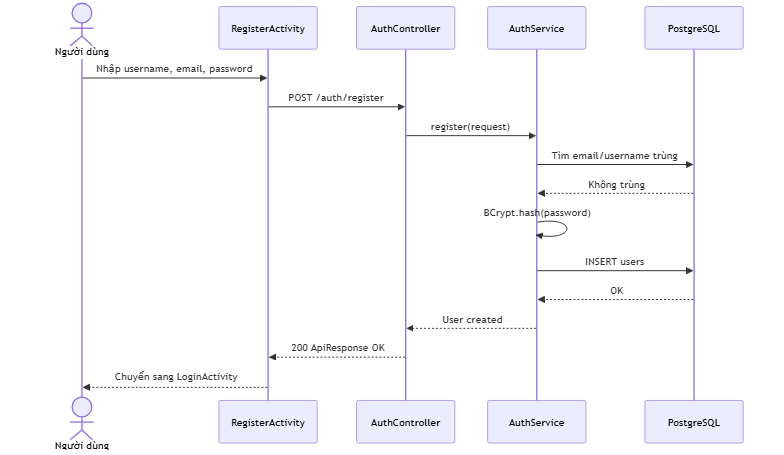
\includegraphics[width=0.9\textwidth]{figures/outputs/seq/UC-01.png}
    \caption{Sơ đồ Tuần tự: UC-01 Đăng ký tài khoản}
    \label{fig:seq_uc_01}
\end{figure}

\textbf{2. UC-02: Đăng nhập hệ thống}
\begin{figure}[H]
    \centering
    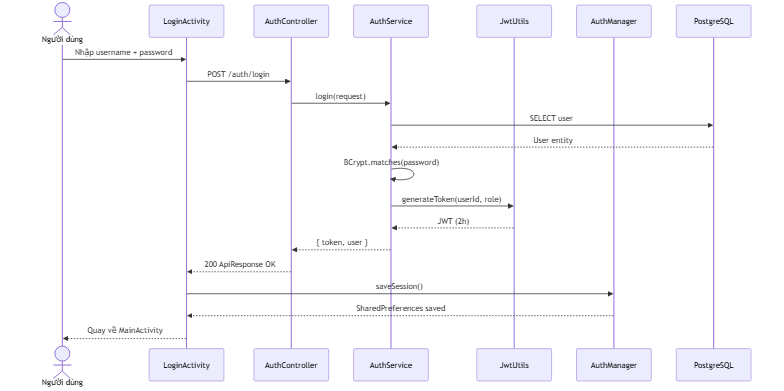
\includegraphics[width=0.9\textwidth]{figures/outputs/seq/UC-02.png}
    \caption{Sơ đồ Tuần tự: UC-02 Đăng nhập hệ thống}
    \label{fig:seq_uc_02}
\end{figure}

\textbf{3. UC-03: Quên mật khẩu}
\begin{figure}[H]
    \centering
    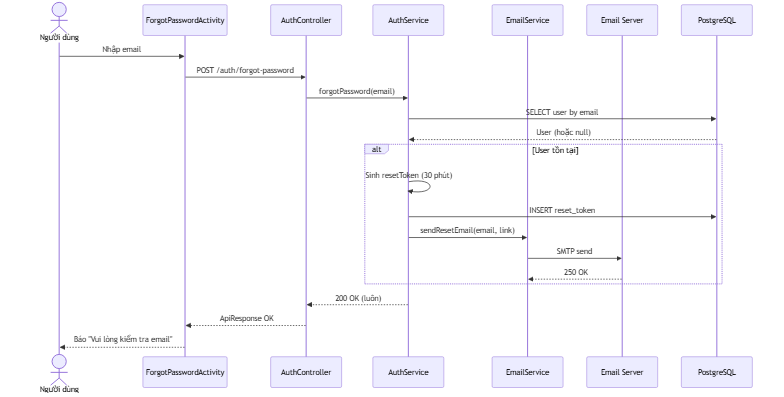
\includegraphics[width=0.9\textwidth]{figures/outputs/seq/UC-03.png}
    \caption{Sơ đồ Tuần tự: UC-03 Quên mật khẩu}
    \label{fig:seq_uc_03}
\end{figure}

\textbf{4. UC-04: Đặt lại mật khẩu}
\begin{figure}[H]
    \centering
    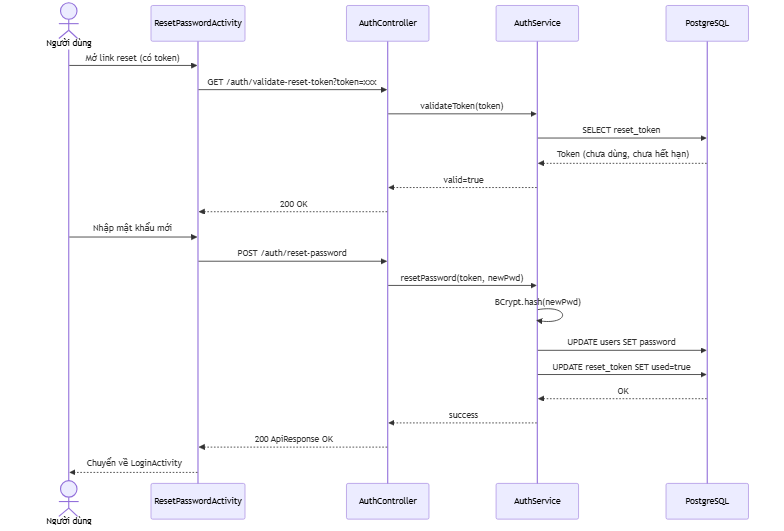
\includegraphics[width=0.9\textwidth]{figures/outputs/seq/UC-04.png}
    \caption{Sơ đồ Tuần tự: UC-04 Đặt lại mật khẩu}
    \label{fig:seq_uc_04}
\end{figure}

\textbf{5. UC-05: Đăng xuất}
\begin{figure}[H]
    \centering
    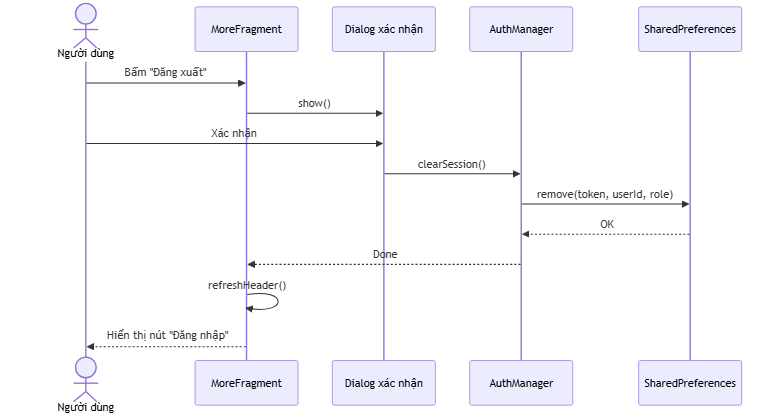
\includegraphics[width=0.9\textwidth]{figures/outputs/seq/UC-05.png}
    \caption{Sơ đồ Tuần tự: UC-05 Đăng xuất}
    \label{fig:seq_uc_05}
\end{figure}

\textbf{6. UC-06: Xem trang chủ}
\begin{figure}[H]
    \centering
    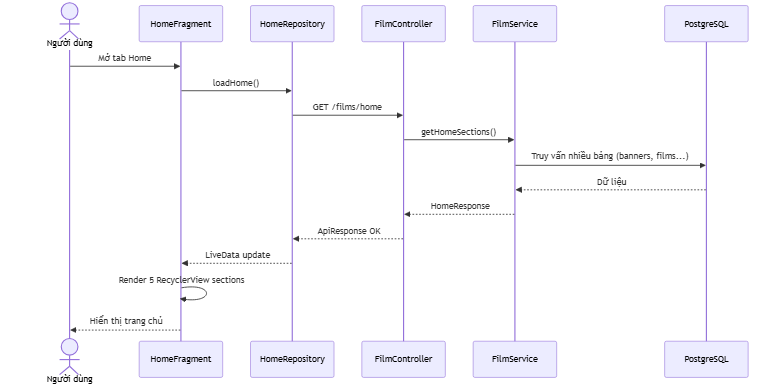
\includegraphics[width=0.9\textwidth]{figures/outputs/seq/UC-06.png}
    \caption{Sơ đồ Tuần tự: UC-06 Xem trang chủ}
    \label{fig:seq_uc_06}
\end{figure}

\textbf{7. UC-07: Xem chi tiết phim}
\begin{figure}[H]
    \centering
    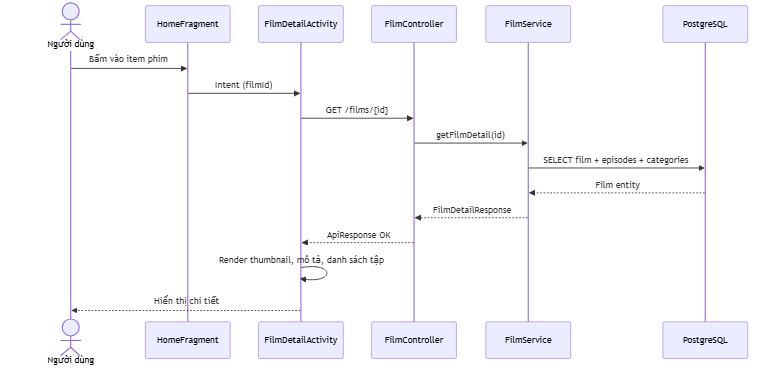
\includegraphics[width=0.9\textwidth]{figures/outputs/seq/UC-07.png}
    \caption{Sơ đồ Tuần tự: UC-07 Xem chi tiết phim}
    \label{fig:seq_uc_07}
\end{figure}

\textbf{8. UC-08: Phát video}
\begin{figure}[H]
    \centering
    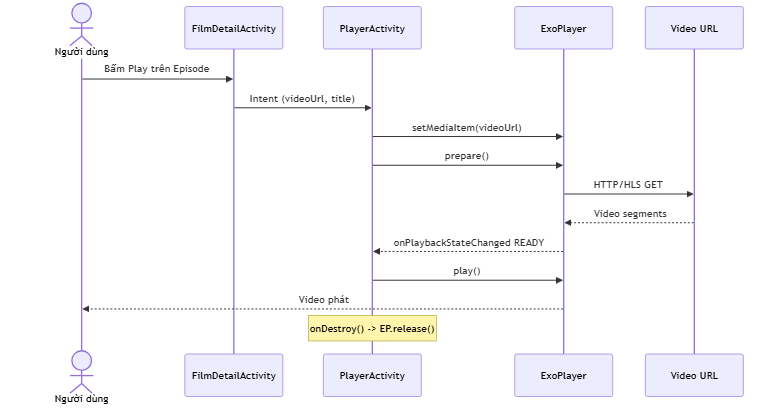
\includegraphics[width=0.9\textwidth]{figures/outputs/seq/UC-08.png}
    \caption{Sơ đồ Tuần tự: UC-08 Phát video}
    \label{fig:seq_uc_08}
\end{figure}

\textbf{9. UC-09: Xem video ngắn (Shorts)}
\begin{figure}[H]
    \centering
    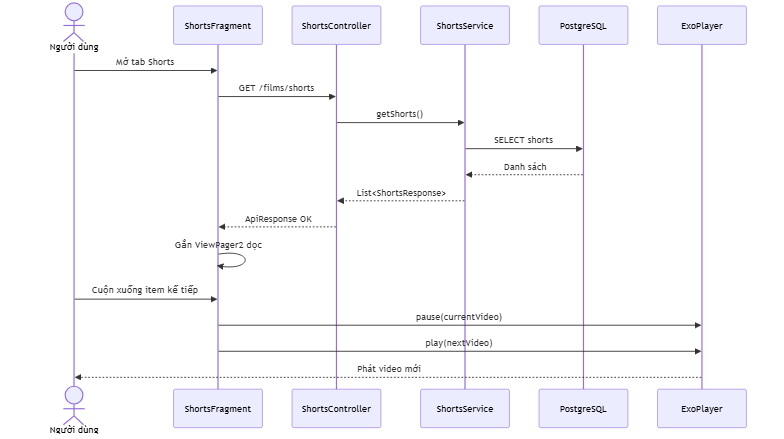
\includegraphics[width=0.9\textwidth]{figures/outputs/seq/UC-09.png}
    \caption{Sơ đồ Tuần tự: UC-09 Xem video ngắn}
    \label{fig:seq_uc_09}
\end{figure}

\textbf{10. UC-10: Xem lịch Premier League}
\begin{figure}[H]
    \centering
    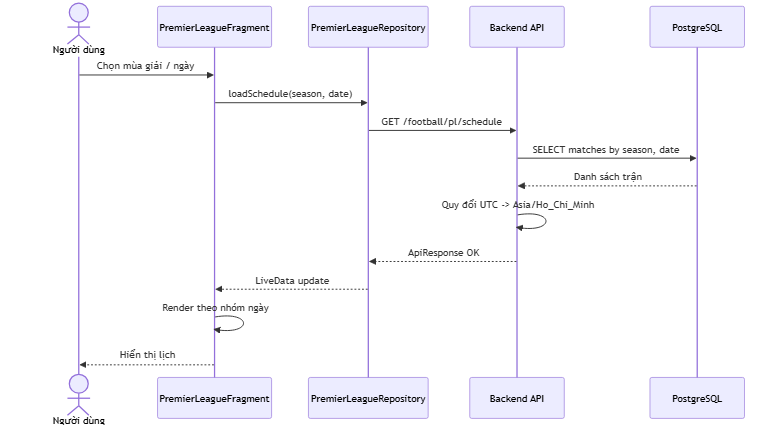
\includegraphics[width=0.9\textwidth]{figures/outputs/seq/UC-10.png}
    \caption{Sơ đồ Tuần tự: UC-10 Xem lịch Premier League}
    \label{fig:seq_uc_10}
\end{figure}

\textbf{11. UC-11: Xem Dashboard quản trị}
\begin{figure}[H]
    \centering
    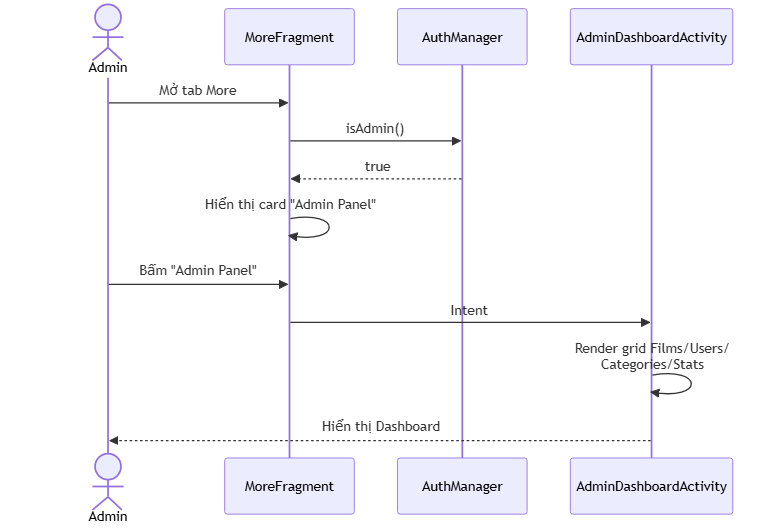
\includegraphics[width=0.9\textwidth]{figures/outputs/seq/UC-11.png}
    \caption{Sơ đồ Tuần tự: UC-11 Xem Dashboard quản trị}
    \label{fig:seq_uc_11}
\end{figure}

\textbf{12. UC-12: Tạo phim mới}
\begin{figure}[H]
    \centering
    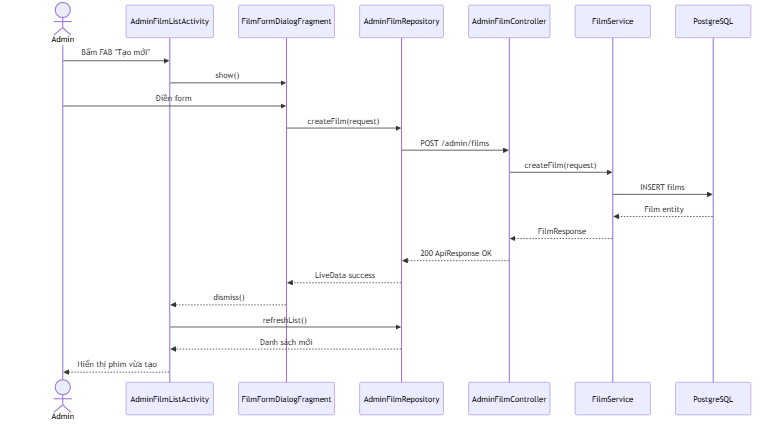
\includegraphics[width=0.9\textwidth]{figures/outputs/seq/UC-12.png}
    \caption{Sơ đồ Tuần tự: UC-12 Tạo phim mới}
    \label{fig:seq_uc_12}
\end{figure}

\textbf{13. UC-13: Cập nhật phim}
\begin{figure}[H]
    \centering
    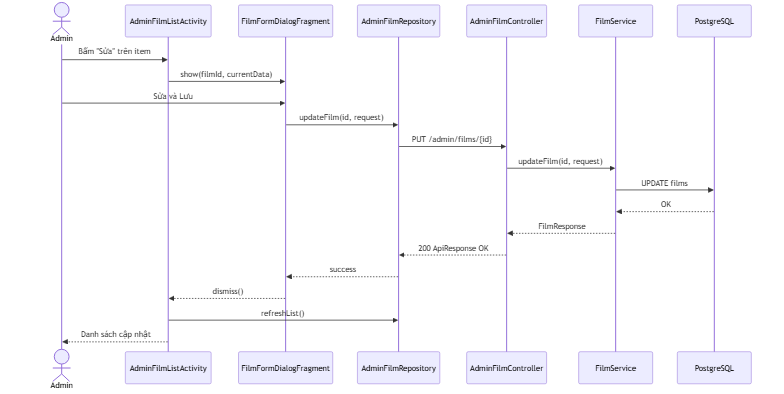
\includegraphics[width=0.9\textwidth]{figures/outputs/seq/UC-13.png}
    \caption{Sơ đồ Tuần tự: UC-13 Cập nhật phim}
    \label{fig:seq_uc_13}
\end{figure}

\textbf{14. UC-14: Xoá phim}
\begin{figure}[H]
    \centering
    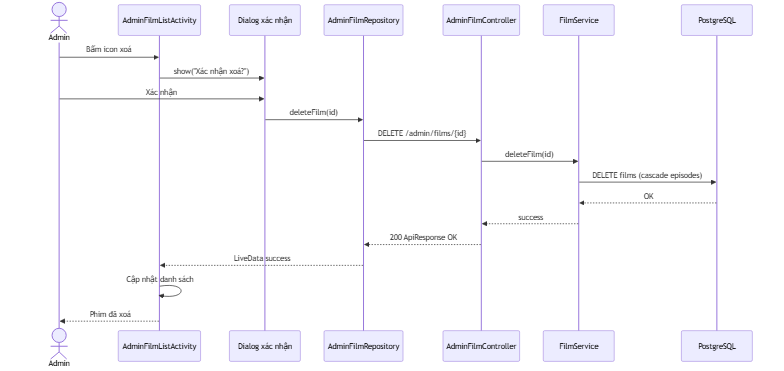
\includegraphics[width=0.9\textwidth]{figures/outputs/seq/UC-14.png}
    \caption{Sơ đồ Tuần tự: UC-14 Xoá phim}
    \label{fig:seq_uc_14}
\end{figure}

\textbf{15. UC-15: Quản lý danh mục thể loại}
\begin{figure}[H]
    \centering
    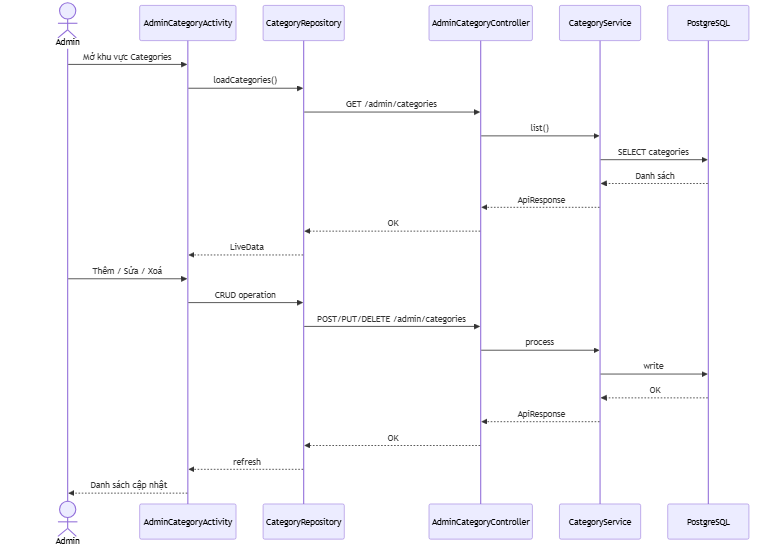
\includegraphics[width=0.9\textwidth]{figures/outputs/seq/UC-15.png}
    \caption{Sơ đồ Tuần tự: UC-15 Quản lý danh mục thể loại}
    \label{fig:seq_uc_15}
\end{figure}



% ────────────────────────────────────────────────────────────
\section{Kiến trúc tổng thể}
\label{sec:kien_truc}

% ── 3.1 Sơ đồ kiến trúc tổng thể ───────────────────────────
\subsection{Sơ đồ Kiến trúc Tổng thể}
\label{subsec:so_do_kien_truc}

Kiến trúc của hệ thống CineFlow được thiết kế theo mô hình \textbf{Client--Server}
truyền thống nhưng có phân lớp chặt chẽ ở cả hai phía. Việc lựa chọn kiến trúc đơn
khối thay vì Microservices xuất phát từ thực tế của dự án:
\begin{itemize}
  \item Phạm vi nghiệp vụ của một ứng dụng xem phim ở mức môn học không đủ phức tạp
  để biện minh cho chi phí vận hành của Microservices (nhiều service, nhiều database,
  message broker, observability\dots).
  \item Đội ngũ phát triển là sinh viên, ưu tiên một mô hình dễ triển khai, dễ debug
  và dễ trình bày trong báo cáo.
\end{itemize}

Hệ thống được chia thành các thành phần cốt lõi như sau:

\begin{enumerate}
  \item \textbf{Android Client:} Ứng dụng native viết bằng Java, giao tiếp với
  backend hoàn toàn qua REST API.
  \item \textbf{Spring Boot Backend:} Tổ chức theo ba tầng cổ điển
  \textit{Controller} -- \textit{Service} -- \textit{Repository}, cung cấp REST API
  với tiền tố \texttt{/api/v1}.
  \item \textbf{PostgreSQL Database:} Lưu toàn bộ dữ liệu nghiệp vụ. Schema được
  quản lý bằng Flyway.
  \item \textbf{Email Server (SMTP):} Đóng vai trò ngoại vi cho luồng khôi phục mật
  khẩu, được backend gọi qua Spring Mail.
  \item \textbf{Content Delivery (URL bên ngoài):} Backend không lưu file video mà
  chỉ lưu URL trỏ tới các nguồn video bên ngoài (ví dụ Google Cloud Storage, S3
  hoặc CDN), ExoPlayer streaming trực tiếp từ các URL này.
\end{enumerate}

\begin{figure}[H]
  \centering
  
\includegraphics[width=0.9\textwidth, height=10cm, keepaspectratio]{outputs/system_arch.png}
  \caption{Sơ đồ Kiến trúc Tổng thể của hệ thống CineFlow}
  \label{fig:system_arch}
\end{figure}

Sơ đồ trên (Hình~\ref{fig:system_arch}) minh hoạ rõ ràng sự phân chia ba luồng giao
tiếp: luồng REST API đồng bộ từ client tới backend, luồng truy vấn JDBC từ backend
tới PostgreSQL, và luồng SMTP từ backend tới email server. Phía Android client tự
phân lớp UI -- Repository -- Network, đảm bảo các Fragment/Activity không bao giờ
gọi trực tiếp Retrofit.

% ── 3.2 Cơ chế giao tiếp ────────────────────────────────
\subsection{Cơ chế giao tiếp Client--Server}
\label{subsec:communication}

Để đảm bảo ứng dụng phản hồi mượt mà ngay cả khi mạng di động không ổn định, toàn bộ
luồng giao tiếp được chia làm ba cơ chế thiết kế chuyên biệt:

\begin{itemize}
  \item \textbf{Giao tiếp Đồng bộ HTTP/REST:} Mọi thao tác đọc/ghi nghiệp vụ đều đi
  qua một tập endpoint REST với tiền tố \texttt{/api/v1}. Android client sử dụng
  Retrofit để khai báo endpoint dưới dạng interface Java; OkHttp đảm nhận kết nối
  HTTP thực tế. Dù gọi là "đồng bộ" về mặt giao thức (request-response), mọi lệnh
  gọi đều được phát đi bất đồng bộ trên luồng nền bằng \texttt{Call.enqueue()} để
  không chặn UI thread.

  \item \textbf{Tự động đính kèm xác thực (Interceptor):} Đồ án cài đặt một
  \texttt{AuthInterceptor} ở tầng OkHttp. Trước mỗi request, interceptor đọc JWT
  được lưu trong \texttt{SharedPreferences} và đính kèm vào header
  \texttt{Authorization: Bearer <token>}. Tầng nghiệp vụ tuyệt đối không cần can
  thiệp vào logic xác thực, đảm bảo nguyên tắc DRY và giảm nguy cơ quên đính kèm
  token.

  \item \textbf{Phát Video Streaming (Direct HTTP/HLS):} Khác với dữ liệu nghiệp
  vụ, luồng video không đi qua backend mà được ExoPlayer streaming trực tiếp từ
  URL nguồn (HTTP hoặc HLS). Backend chỉ trả về URL trong DTO của \texttt{Episode}.
  Thiết kế này giảm tải đáng kể cho backend và tận dụng được hạ tầng CDN của nhà
  cung cấp nội dung.
\end{itemize}

\subsubsection{Bản đồ Giao tiếp Cụ thể trong các Luồng nghiệp vụ}
Để làm rõ cơ chế trên, dưới đây là bản đồ giao tiếp thực tế của hai luồng nghiệp
vụ tiêu biểu của ứng dụng CineFlow.

\paragraph{1. Luồng Xác thực và Duy trì Phiên đăng nhập}
\mbox{}\\
Luồng này phục vụ việc xác thực người dùng và duy trì phiên trong các phiên làm
việc tiếp theo.

\begin{figure}[H]
  \centering
  
\includegraphics[width=0.85\textwidth, height=7cm, keepaspectratio]{outputs/auth_comm.png}
  \caption{Sơ đồ Tuần tự minh hoạ luồng đăng nhập và đính kèm JWT}
  \label{fig:auth_comm}
\end{figure}

Khi người dùng đăng nhập thành công, backend trả về JWT có thời hạn 2 giờ. Android
client lưu token và thông tin user vào \texttt{SharedPreferences} thông qua
\texttt{AuthManager}. Ở các request tiếp theo, \texttt{AuthInterceptor} tự động
đính kèm token mà không cần Fragment/Activity can thiệp.

\paragraph{2. Luồng Phát Video Streaming}
\mbox{}\\
Đại diện cho luồng tách biệt giữa dữ liệu nghiệp vụ và nội dung media.

\begin{figure}[H]
  \centering
  
\includegraphics[width=0.85\textwidth, height=7cm, keepaspectratio]{outputs/play_video_comm.png}
  \caption{Sơ đồ Tuần tự minh hoạ luồng phát video streaming}
  \label{fig:play_video_comm}
\end{figure}

Khi người dùng bấm Play trên \texttt{FilmDetailActivity}, client gọi \texttt{GET
/films/\{id\}} để lấy danh sách \texttt{Episode} kèm \texttt{videoUrl}.
\texttt{PlayerActivity} được mở qua \texttt{Intent}, khởi tạo \texttt{ExoPlayer}
và bắt đầu streaming trực tiếp từ URL nguồn -- backend hoàn toàn không tham gia
vào luồng truyền dữ liệu video.


% ── 3.3 Áp dụng mẫu thiết kế ────────────────────────────────
\subsection{Áp dụng Mẫu thiết kế (Design Patterns)}
\label{subsec:design_patterns}

Hệ thống CineFlow áp dụng nhiều mẫu thiết kế hướng đối tượng (Object-Oriented Design
Patterns) ở cả hai phía Android và Backend nhằm đảm bảo mã nguồn dễ bảo trì, dễ mở
rộng và phù hợp với chuẩn mực của lập trình di động.

\subsubsection{Các Mẫu Thiết kế Phía Android}

\paragraph{1. Repository Pattern}
\mbox{}\\
Tầng giao diện (Fragment/Activity) không trực tiếp gọi Retrofit hay truy cập cache.
Thay vào đó, mỗi miền dữ liệu được phơi qua một lớp Repository riêng
(\texttt{HomeRepository}, \texttt{AdminFilmRepository},
\texttt{PremierLeagueRepository}). Repository đóng gói toàn bộ chi tiết tầng mạng
và trả kết quả qua \texttt{LiveData}. Nhờ đó, khi thay đổi nguồn dữ liệu (ví dụ
thêm cache local), tầng UI hoàn toàn không bị ảnh hưởng.

\paragraph{2. Singleton Pattern}
\mbox{}\\
Các thành phần dùng chung toàn cục như \texttt{ApiClient} (Retrofit instance),
\texttt{AuthManager} (truy cập \texttt{SharedPreferences}) và mỗi Repository đều
được hiện thực dưới dạng Singleton. Singleton đảm bảo chỉ có duy nhất một instance
trong toàn bộ vòng đời ứng dụng -- tiết kiệm tài nguyên (đặc biệt là kết nối
OkHttp pool) và tránh sai lệch trạng thái khi nhiều Fragment cùng truy cập.

\paragraph{3. Adapter Pattern}
\mbox{}\\
\texttt{RecyclerView} của Android tuân theo \textbf{Adapter Pattern} một cách tự
nhiên: \texttt{RecyclerView.Adapter} là cầu nối giữa dữ liệu (danh sách phim,
shorts, lịch thi đấu) và view item. CineFlow tận dụng pattern này để hiển thị
hàng chục loại danh sách khác nhau (banner ngang, hàng phim mới, danh sách quản
trị\dots) mà không trùng lặp mã nguồn UI.

\paragraph{4. Interceptor Pattern}
\mbox{}\\
\texttt{AuthInterceptor} là minh hoạ điển hình của \textbf{Interceptor Pattern}
trên Android. Interceptor chặn mọi request trước khi gửi đi, thêm header
\texttt{Authorization} và để cho phần còn lại của hệ thống tiếp tục như không có
gì xảy ra. Pattern này hiện thực ý tưởng \textit{cross-cutting concern} (xác thực)
mà không làm bẩn logic nghiệp vụ.

\paragraph{5. Observer Pattern (qua LiveData)}
\mbox{}\\
\texttt{LiveData} của Android là một hiện thực có lifecycle-awareness của
\textbf{Observer Pattern}. Repository phơi dữ liệu dưới dạng \texttt{LiveData};
Fragment đăng ký quan sát bằng \texttt{observe()}. Khi dữ liệu thay đổi, UI tự
cập nhật; khi Fragment bị huỷ, đăng ký tự động được dọn dẹp -- triệt tiêu một
trong những nguồn rò rỉ bộ nhớ phổ biến nhất trên Android.

\paragraph{6. Template Method Pattern (qua BaseFragment)}
\mbox{}\\
\texttt{BaseFragment} định nghĩa khung lifecycle chuẩn với ba phương thức trừu
tượng \texttt{getLayoutId()}, \texttt{initViews()}, \texttt{initData()}. Các
Fragment con chỉ cần cài đặt ba phương thức này, phần điều phối còn lại (gọi
\texttt{inflate}, gọi \texttt{initViews} trước \texttt{initData}) được lớp cha
xử lý tập trung. Đây chính là \textbf{Template Method Pattern} kinh điển.

\subsubsection{Các Mẫu Thiết kế Phía Backend}

\paragraph{1. Layered Architecture (3 tầng)}
\mbox{}\\
Backend tổ chức rõ rệt ba tầng: \texttt{Controller} (mở endpoint REST, validate
dữ liệu vào, trả \texttt{ApiResponse<T>}); \texttt{Service} (chứa logic nghiệp
vụ, transaction); \texttt{Repository} (giao tiếp PostgreSQL qua Spring Data JPA).
Mỗi tầng chỉ phụ thuộc tầng ngay bên dưới, cho phép thay thế hoặc kiểm thử độc
lập từng tầng.

\paragraph{2. DTO Pattern \& Unified Response Envelope}
\mbox{}\\
Không bao giờ trả thẳng Entity ra ngoài API. Mọi response đều đi qua một lớp DTO
chuyên biệt (\texttt{FilmResponse}, \texttt{UserResponse}\dots) rồi được bọc
trong vỏ chung \texttt{ApiResponse<T>} (gồm \texttt{success}, \texttt{message},
\texttt{data}). Client Android chỉ cần phân tích cú pháp một cấu trúc duy nhất
cho toàn bộ hệ thống.

\paragraph{3. Filter Chain (Spring Security)}
\mbox{}\\
Mọi request đi vào backend đều đi qua \textbf{Filter Chain} của Spring Security.
\texttt{AuthTokenFilter} đứng trước \texttt{UsernamePasswordAuthenticationFilter},
giải mã JWT, kiểm tra chữ ký và bơm \texttt{Authentication} vào
\texttt{SecurityContext}. Tầng Controller chỉ cần dùng annotation
\texttt{@AuthenticationPrincipal} để lấy user hiện tại -- không bao giờ phải tự
parse JWT.

\paragraph{4. Strategy Pattern (gửi email)}
\mbox{}\\
\texttt{EmailService} đóng vai trò một Strategy cho các luồng cần gửi email (khôi
phục mật khẩu, thông báo). Phía sau cùng một interface, ta có thể đổi sang
SendGrid, Mailgun hay Amazon SES mà không phải sửa Service nghiệp vụ.

\paragraph{5. Migration Pattern (Flyway)}
\mbox{}\\
Việc quản lý schema bằng các file \texttt{V<N>\_\_*.sql} có đánh số tuần tự là
một mẫu kiến trúc đặc thù cho ứng dụng có database: schema được coi như mã nguồn
-- có lịch sử, có thể review và có thể tái lập lại trên mọi môi trường.


% ────────────────────────────────────────────────────────────
\section{Thiết kế cấu hình các node và mạng}
\label{sec:cau_hinh_node}

Hệ thống CineFlow được thiết kế để triển khai linh hoạt trên cả môi trường phát
triển cục bộ (máy thành viên + emulator) lẫn môi trường thử nghiệm (máy server +
thiết bị Android thật). Cấu trúc liên kết mạng và cấu hình các Node được phân
định rõ ràng để đảm bảo có thể chuyển đổi giữa hai môi trường mà chỉ cần thay đổi
một biến cấu hình.

\begin{figure}[H]
  \centering
  
\includegraphics[width=\textwidth, height=12cm, keepaspectratio]{outputs/deployment_arch.png}
  \caption{Sơ đồ Triển khai (Deployment Diagram) các Node và Phân vùng mạng}
  \label{fig:deployment_arch}
\end{figure}

\subsection{Cấu trúc Phân vùng Mạng}
Hệ thống mạng được thiết lập thành 3 ranh giới rõ rệt:
\begin{itemize}
  \item \textbf{Mạng thiết bị di động (Mobile Network):} Nơi thiết bị Android (hoặc
  emulator) hoạt động, giao tiếp với backend qua HTTP/HTTPS.
  \item \textbf{Mạng Backend (Application Network):} Nơi đặt ứng dụng Spring Boot.
  Trong môi trường phát triển, backend chạy trên \texttt{localhost:8080}; trong môi
  trường thử nghiệm, backend được đóng gói thành JAR và chạy sau Reverse Proxy
  (Nginx) qua HTTPS.
  \item \textbf{Mạng Dữ liệu (Data Network):} Nơi PostgreSQL chạy. Trong dự án này,
  PostgreSQL được khởi động qua Docker Compose (\texttt{compose.yml}), tự cô lập
  trong mạng nội bộ Docker, chỉ mở cổng \texttt{5432} cho backend.
\end{itemize}

\subsection{Cấu hình Môi trường Phát triển}
Trong môi trường phát triển cục bộ:
\begin{itemize}
  \item Backend chạy trên \texttt{localhost:8080}, kết nối PostgreSQL qua
  \texttt{jdbc:postgresql://localhost:5432/mydb}.
  \item Android emulator truy cập backend qua địa chỉ \texttt{10.0.2.2:8080} --
  đây là alias mặc định của máy chủ host nhìn từ trong emulator. Nhờ alias này,
  toàn bộ dự án có thể chạy thử nghiệm hoàn toàn cục bộ mà không cần triển khai
  lên server.
  \item Các biến nhạy cảm (\texttt{JWT\_SECRET}, \texttt{MAIL\_USERNAME},
  \texttt{MAIL\_PASSWORD}) được nạp qua biến môi trường, không commit vào Git.
  Mật khẩu PostgreSQL chỉ dùng cho môi trường phát triển và được khai báo trong
  \texttt{compose.yml}.
\end{itemize}

\subsection{Cấu hình cho Thiết bị Android Thật}
Khi cần kiểm thử trên thiết bị Android thật:
\begin{itemize}
  \item Thiết bị Android và máy chủ backend phải nằm trong cùng một mạng LAN.
  \item Sửa \texttt{ApiClient.BASE\_URL} từ \texttt{http://10.0.2.2:8080/api/v1/}
  thành địa chỉ IP nội bộ của máy chủ (ví dụ \texttt{http://192.168.1.10:8080/api/v1/}).
  \item Cần khai báo \texttt{android:usesCleartextTraffic="true"} trong
  \texttt{AndroidManifest.xml} hoặc thiết lập \texttt{network\_security\_config.xml}
  để Android chấp nhận HTTP plaintext (vì môi trường thử nghiệm chưa có HTTPS).
\end{itemize}

Thiết kế tách bạch \texttt{BASE\_URL} như trên cho phép chuyển nhanh giữa các môi
trường mà không phải sửa code nghiệp vụ.
